\documentclass[12pt, a4paper]{report}
\usepackage[utf8]{inputenc}
\newcommand\preamble{
    \usepackage[italian]{babel}
    \usepackage{geometry}
    \usepackage{amsmath}
    \usepackage{amssymb}
    \usepackage{graphicx}
    \usepackage{ulem}
    \usepackage[dvipsnames]{xcolor}

    \geometry{margin=2cm}
    \let\olditemize\itemize
    \renewcommand\itemize{\olditemize\setlength\itemsep{0em}}
    \graphicspath{{../Immagini/}}

    \author{Lorenzo Vaccarecci}
}
\preamble

\usepackage{lipsum} 
\usepackage{caption}
\usepackage{fancyhdr}
\usepackage{setspace}
\usepackage{titlesec}

\geometry{top=1in, bottom=1in, left=1in, right=1in}

\pagestyle{fancy}
\fancyhf{}
\rfoot{\thepage}
\renewcommand{\headrulewidth}{0pt}

\titleformat{\chapter}[display]
  {\normalfont\fontsize{14}{16}\selectfont\bfseries\centering}{\MakeUppercase{\chaptertitlename}\ \thechapter}{20pt}{\fontsize{14}{16}\selectfont\bfseries}
\titleformat{\section}
  {\normalfont\fontsize{12}{14}\selectfont\bfseries}{\thesection}{1em}{}
\titleformat{\subsection}
  {\normalfont\fontsize{12}{14}\selectfont\bfseries}{\thesubsection}{1em}{}
\titleformat{\subsubsection}
  {\normalfont\fontsize{12}{14}\selectfont\bfseries}{\thesubsubsection}{1em}{}

  \makeatletter
  \renewcommand*\l@chapter[2]{%
    \ifnum \c@tocdepth >\m@ne
      \addpenalty{-\@highpenalty}%
      \vskip 1.0em \@plus\p@
      \setlength\@tempdima{1.5em}%
      \begingroup
        \parindent \z@ \rightskip \@pnumwidth
        \parfillskip -\@pnumwidth
        \leavevmode \bfseries
        \advance\leftskip\@tempdima
        \hskip -\leftskip
        #1\nobreak\hfil \nobreak\hb@xt@\@pnumwidth{\hss #2}\par
        \penalty\@highpenalty
      \endgroup
    \fi}
  
  \renewcommand*\l@section{\@dottedtocline{1}{0em}{2.3em}}
  \renewcommand*\l@subsection{\@dottedtocline{2}{2.3em}{3.2em}}
  \renewcommand*\l@subsubsection{\@dottedtocline{3}{5.5em}{4.1em}}
  \renewcommand*\l@paragraph{\@dottedtocline{4}{8.6em}{5em}}
  \renewcommand*\l@subparagraph{\@dottedtocline{5}{12em}{6em}}
  \makeatother 

\begin{document}
    \begin{titlepage}
        \centering
        % Title
        {\Huge \bfseries{[Appunti Basi di Dati]}\par}
        \vspace{1cm}
        {\large Appunti del corso "Basi di Dati" dell'Università degli Studi di Genova\par}
        {\Large\bfseries Lorenzo Vaccarecci\par}
        \vspace{1cm}
        % University Logo
        
\includegraphics[width=0.7\textwidth]{Appunti Latex/Immagini/logoUnige.png}\\
        \vspace{1cm}
        % Department and University
        {\Large\bfseries Dipartimento di Informatica\par}
        {\Large\bfseries Università degli Studi di Genova\par}
        {\Large\bfseries 2024\par}
    \end{titlepage}
    \tableofcontents
    \chapter{Modello Relazionale}
        \section{Introduzione}
            Le interrogazioni sulle relazioni possono essere espresse in due formalismi:
            \begin{itemize}
                \item \textbf{Algebra relazionale}: le interrogazioni vengono espresse usando operatori specifici alle relazioni.
                \item \textbf{Calcolo relazionale}: le interrogazioni vengono espresse usando formule logiche.
            \end{itemize}
        \section{Relazioni}
            Un dominio è un insieme (anche infinito) di valori. Indicheremo con $\mathcal{D}$ l'insieme di tutti i domini.
            \subsection{Definizione: Prodotto cartesiano}
                Siano $D_{1},D_{2},\ldots,D_{k} \in \mathcal{D} \text{ con } k$ domini. Il prodotto cartesiano indicato con $D_{1}\times D_{2}\times \ldots \times D_{k}$, è definito come l'insieme $\left\{\left(v_{1},v_{2},\ldots,v_{k}\right)|v_{1}\in D_{1},\ldots,v_{k}\in D_{k}\right\}$.\\
                Gli elementi appartenenti al prodotto cartesiano sono detti \important{tuple}. Il prodotto cartesiano ha \textbf{grado} $k$.
            \subsection{Definizione: Relazione}
                Una relazione di $k$ domini è un sottoinsieme finito del prodotto cartesiano, ha \textbf{grado} $k$ quindi ogni tupla ha $k$ componenti. La \textbf{cardinalità} di una relazione è il numero di tuple appartenenti alla relazione. Una relazione è \underline{sempre} un insieme finito. \remark{Non vi sono tuple duplicate}.\\
            La coppia (nome di attributo, dominio) è detta \important{attributo}. L'uso di attributi permette di denotare le componenti di ogni tupla per nome piuttosto che per posizione.
            \subsection{Definizione: Schema di relazione}
                \begin{itemize}
                    \item $R$ un nome di relazione
                    \item $\left\{A_{1},A_{2},\ldots,A_{n}\right\}$ un insieme di nomi di attributi
                    \item $dom:\left\{A_{1},A_{2},\ldots,A_{n}\right\}\rightarrow \mathcal{D}$ una funzione totale che associa ad ogni nome di attributo il corrispondente dominio.
                \end{itemize}
                La coppia $(R(A_{1},A_{2},\ldots,A_{n}),dom)$ è uno schema di relazione. $U_{r}$ denota l'insieme dei nomi di attributi di $R$, ovvero \important{$U_{r}=\left\{A_{1},A_{2},\ldots,A_{n}\right\}$}.
            \subsection{Definizione: Schema di base di dati}
                Siano $S_{1},S_{2},\ldots,S_{n}$ schemi di relazioni distinti, $\mathcal{S}=\left\{S_{1},S_{2},\ldots,S_{n}\right\}$ è detto schema di base di dati.
            \subsection{Definizione: Tuple e relazione}
                Una tupla $t$ definita su una relazione $R$ è un insieme di funzioni totali che associano all'attributo di nome $A_{i}$ un valore del dominio di tale attributo. Una relazione definita su uno schema di relazione è un insieme finito di tuple definite su tale schema. Tale relazione è anche detta istanza dello schema. $t=\left[A_{1}:v_{1},A_{2}:v_{2},\ldots,A_{n}:v_{n}\right]$ dove $v_{i}\in dom(A_{i}) \text{ con } i=1,\ldots,n$. Notazione: $t[A_{i}]$ indica il valore dell'attributo $A_{i}$(quindi $v_{i}$) nella tupla $t$.
        \section{Valori nulli}
            Un aspetto importante nella modellazione dei dati riguarda il fatto che non sempre sono disponibili tutte le informazioni sulle entità del dominio applicativo che vengono rappresentate nella base di dati. L'approccio adottato è quello di introdurre un valore speciale, detto \important{valore nullo}, il quale denota la mancanza di un valore.\\
            Nella trattazione assumiamo di denotare il valore nullo con il simbolo '\texttt{?}'. Il valore nullo è un valore accettato in tutti i domini.
        \section{Chiavi}
            Una \important{chiave} di una relazione è un insieme di attributi che distingue fra loro le tuple della relazione. Più formalmente:
            \subsection{Definizione: Chiave e super-chiave}
                Sia $R$ uno schema di relazione. Un insieme $X\subseteq U_{R}$ di attributi di $R$ è chiave di $R$ se verifica le seguenti proprietà:
                \begin{enumerate}
                    \item \important{Univocità}: nella relazione non ci possono essere due tuple distinte che abbiano lo stesso valore per tutti gli attributi della chiave $X$.
                    \item Nessun \textbf{sottoinsieme proprio} di $X$ verifica la proprietà (1).
                \end{enumerate}
                Un insieme di attributi che verifica la proprietà (1) ma non la (2) è detto \important{super-chiave} di $R$. Una super-chiave può essere una chiave della relazione.\\
                In una relazione ci possono essere più insiemi di attributi che soddisfano le due proprietà. In tal caso si parla di \important{chiavi candidate}. \textbf{Una relazione ha sicuramente almeno una chiave (sia primaria che super)}. Nel caso in cui ci sono più chiavi candidate, una di queste viene scelta come \important{chiave primaria} su cui il DBMS ottimizza le operazioni.\\
                Un criterio per scegliere la chiave primaria è quello di scegliere la chiave più piccola in termini di numero di attributi o quella più usata nelle interrogazioni. Una chiave non può contenere valori nulli.
            \subsection{Definizione: Chiave esterna}
                Sia $R_{1}$ ed $R_{2}$ due relazioni, sia $X$ una chiave per $R_{1}$ e $Y$ una chiave per $R_{2}$ tale che $Y$ e $X$ contengano lo stesso numero di attributi e di dominio compatibile (\textit{es. interi e reali sono compatibili}). $X$ è una chiave esterna di $R_{1}$ su $R_{2}$ se per ogni tupla $t$ di $R_{1}$ esiste una tupla $t'$ di $R_{2}$ tale che $t[X]=t'[Y]$. $R_{1}$ viene detta relazione \textbf{referente} e $R_{2}$ relazione \textbf{riferita}.\\
                \remark{Vincolo di integrità refernziale}: se una tupla $t$ di $R_{1}$ fa riferimento ai valori della chiave di una tupla $t'$ di $R_{2}$, allora $t'$ deve esistere in $R_{2}$. Può essere violata da inserimenti e modifiche nella relazione referente e da cancellazioni e modifiche nella relazione riferita.\\
                Una relazione può contenere più chiavi esterne, eventualmente anche sulla stessa relazione e possono assumere valori nulli.\\
                \textbf{Notazione:}
                \begin{equation*}
                    R_{1}\left(\dots,chiave\_esterna^{R_{2}},\dots\right)
                \end{equation*}
    \chapter{Modello ER}
    \section{Introduzione}
    Il termine \important{diagramma ER} indica la rappresentazione grafica di uno schema concettuale ER.
    Gli elementi principali di un diagramma ER sono:
    \begin{itemize}
        \item \important{Entità}: una collezione di oggetti della realtà che vogliamo modellare che possiedono caratteristiche comuni, graficamente viene rappresentata da un rettangolo
        \item \important{Relazioni} (o associazione): rappresenta un legame logico tra più entità, graficamente viene rappresentata da un rombo
        \item \important{Attributi}: rappresenta una proprietà posseduta da un'entità o da una relazione, è \remark{mono-valore} se può assumere al più un valore (\textit{es. la matricola di uno studente}), è \remark{multi-valore} altrimenti (\textit{es. i numeri di telefono di un'azienda}). Può essere a sua volta essere formato da \textit{sotto-attributi} rendendolo \remark{composto}, un attributo composto può avere domini di diverso tipo (\remark{domini composti})
    \end{itemize}
    \begin{center}
        \begin{tikzpicture}[node distance=4.7em]
            \node[entity] (entity1) {$E_{1}$};
            \node (attr1) [above of = entity1] {A};
            \draw (entity1) -- node[near end, above, draw, circle, minimum size=0.01cm, fill=white] {} (attr1);
            \node[relationship] (rel1) [right of = entity1] {R} edge (entity1);
            \node[entity] (entity2) [right of = rel1] {$E_{2}$} edge (rel1);
            \node[attribute] (attr2) [above of = entity2] {B} edge (entity2);
            \node (attr3) [above of = attr2] {C} edge (attr2);
            \draw (attr2) -- node[near end, above, draw, circle, minimum size=0.01cm, fill=white] {} (attr3);
            \node (attr4) [above left of = attr2] {D} edge (attr2);
            \draw (attr2) -- node[near end, above left, draw, circle, minimum size=0.01cm, fill=white] {} (attr4);
            \node (attr5) [above right of = attr2] {E} edge (attr2);
            \draw (attr2) -- node[near end, above right, draw, circle, minimum size=0.01cm, fill=white] {} (attr5);
        \end{tikzpicture}
    \end{center}
    Le istanze di un'associazione sono un sottoinsieme del prodotto cartesiano delle entità coinvolte, non possono esistere duplicati. Le associazioni sono classificate in base al loro \remark{grado} (il numero di entità in relazione):
    \begin{itemize}
        \item \textbf{Unaria}: un'entità è in relazione con se stessa
        \item \textbf{Binaria}: due entità sono in relazione
        \item \textbf{$n$-aria}: $n$ entità sono in relazione
    \end{itemize}
    Le informazioni sui domini degli attributi non sono direttamente rappresentabili in un diagramma ER, ma possono essere specificate nella documentazione a corredo dei diagrammi ER.
    \section{Vincoli di integrità}
    \subsection{Vincoli di cardinalità}
    I vincoli di cardinalità per associazioni stabiliscono il numero minimo e massimo di istanze di un'associazione a cui le istanze delle entità coinvolte nella associazione possono partecipare. Graficamente, vengono rappresentati come coppia di valori interi $(min,max)$ collocata vicino alla linea che connette l'associazione con ciascuna entità che mette in relazione.
    \begin{center}
        \begin{tikzpicture}[node distance=10em]
            \node[entity] (entity1) {$E_{1}$};
            \node[relationship] (rel1) [right of = entity1] {R};
            \node[entity] (entity2) [right of = rel1] {$E_{2}$};
            \path (entity1) edge node[above]{$(min,max)$} (rel1);
            \path (rel1) edge node[above]{$(min,max)$} (entity2);
        \end{tikzpicture}
    \end{center}
    $(min,max)$:
    \begin{itemize}
        \item $min=0$: l'entità non è obbligata a partecipare all'associazione
        \item $min=1$: l'entità è obbligata a partecipare all'associazione
        \item $max=1$: l'entità può partecipare al massimo una volta all'associazione
        \item $max=n$: l'entità può partecipare al massimo $n$ volte all'associazione
    \end{itemize}
    Se in un diagramma ER non è specificata la cardinalità di un'associazione, si assume che il vincolo sia $(0,n)$.\\
    Date due entità $E_{1}$ e $E_{2}$ se:
    \begin{itemize}
        \item $max_{E_{1}}=max_{E_{2}}=1$ allora l'associazione è \remark{uno a uno}
        \item $max_{E_{1}}=1,max_{E_{2}}=n$ allora l'associazione è \remark{uno a molti}
        \item $max_{E_{1}}=max_{E_{2}}=n$ allora l'associazione è \remark{molti a molti}
    \end{itemize}
    Le cardinalità possono essere specificate anche per gli attributi, permettendo di specificare se un attributo è mono o multi-valore, e se è obbligatorio o meno. Se non viene specificata la cardinalità di un attributo, si assume che sia $(1,1)$.
    \subsection{Vincoli di identificazione}
    Definire un vincolo d'identificazione per un'entità significa specificare un insieme di attributi e/o entità che posseggono la proprietà di identificare univocamente le istanze dell'entità (\important{identificatori o chaivi}).
    \begin{itemize}
        \item \important{Identificatore interno}: è costituito da uno o più attributi dell'entità stessa
        \item \important{Identificatore misto}: è costituito da attributi dell'entità e da attributi di altre entità
        \item \important{Identificatore esterno}: è costituito da attributi di altre entità
        \item \important{Identificatore semplice}: è costituito da un solo attributo
        \item \important{Identificatore composto}: è costituito da più attributi
    \end{itemize}
    Un'entità le cui istanze vengono identificate mediante l'associazione con altre entità viene chiamata \remark{entità debole}.
    \section{Gerarchie di generalizzazione}
    Nel modello ER è possibile organizzare le entità in gerarchia di generalizzazione definendo un insieme di entità dette \remark{figlie} come specializzazione di un'altra entità detta \remark{padre} rappresentante le proprietà in comune a tutte le entità figlie.
    \begin{itemize}
        \item \important{Generalizzazione totale}: ogni istanza dell'entità padre è anche un'istanza di \textbf{almeno} una delle entità figlie
        \item \important{Generalizzazione parziale}: se un'istanza dell'entità padre non è un'istanza di nessuna delle entità figlie
        \item \important{Generalizzazione esclusiva}: se un'istanza dell'entità padre è un'istanza di \textbf{al più} una delle entità figlie
        \item \important{Generalizzazione condivise}: se un'istanza dell'entità padre può essere un'istanza di \textbf{più} entità figlie
    \end{itemize}
    Le generalizzazioni possono essere di quattro tipi diversi: totali esclusive, totali condivise, parziali esclusive e parziali condivise.
    \chapter{Progettazione Logica}
    \section{Introduzione}
    L'obiettivo principale della progettazione logica è tradurre uno schema ER in uno schema relazionale equivalente. Si articola in due fasi:
    \begin{itemize}
        \item \remark{Fase di ristrutturazione dello schema ER}: questa fase prevede l'eliminazione dallo schema ER di tutti quei costrutti non direttamente rappresentabili nel modello relazionale, anche questa fase si può suddividere in più sotto-fasi:
        \begin{itemize}
            \item analisi della ridondanza
            \item partizionamento/accorpamento di entità
            \item eliminazione degli attributi composti e multi-valore
            \item eliminazione delle gerarchie di generalizzazione
        \end{itemize}
        \item \remark{Fase di traduzione dello schema ER}: in questa fase, lo schema ER restituito dalla fase di ristrutturazione viene tradotto in un equivalente schema relazionale. \underline{La traduzione non è sempre univoca}.
    \end{itemize}
    \section{Fase di ristrutturazione}
    \subsection{Analisi della ridondanza}
    Uno schema ER presenta delle ridondanze quando un'informazione viene rappresentata sia esplicitamente nello schema sia può essere derivata da altre informazioni presenti nello schema. Nei diagrammi ER la presenza di ridondanza dovrebbe essere limitata solo a quei casi in cui sia possibile ottenere un significativo beneficio in termini di tempo di esecuzione delle interrogazioni.
    \subsection{Partizionamento/accorpamento di entità}
    Lo schema ER può essere ulteriormente ristrutturato partizionando od accorpando entità ed associazioni sulla base dell'analisi del carico di lavoro. Un'entità $E$ può essere partizionata in due entità $E_{1},E_{2}$ una delle quali identificata esternamente dall'altra, collegate mediante un'associazione uno a uno. Questa operazione può essere conveniente quando alcune operazioni frequenti coinvolgono solo un sottoinsieme degli attributi di $E$. Viceversa, due entità $E_{1},E_{2}$ collegate da un'associazione uno a uno, possono essere accorpate in un'unica entità contenente gli attributi di $E_{1}$ e $E_{2}$ nel caso in cui operazioni frequenti abbiano la necessità di accedere ad entrambi gli insiemi di attributi.
    \subsection{Eliminazione degli attributi composti e multi-valore}
    Il modello relazionale consente la specifica solo di attributi semplici e mono-valore. E' quindi necessario ristrutturare lo schema ER generato dalla fase di progettazione concettuale per eliminare eventuali attributi composti e multi-valore in esso presenti. L'eliminazione di un attributo composto $A$ da un'entità $E$ può avvenite in due modi:
    \begin{itemize}
        \item \remark{Eliminando i sotto-attributi di $A$ e considerando l'attributo composto come un attributo semplice}
        \item \remark{Considerando tutti i sotto-attributi di $A$ come attributi di $E$}
    \end{itemize}
    Quest'ultima soluzione richiede ovviamente una ridefinizione del dominio dell'attributo.\\
    La modellazione di attributi multi-valore mediante attributi a valore semplice richiede la definizione di una nuova entità, collegata all'entità di partenza tramite un'opportuna associazione, in cui l'attributo multi-valore è rappresentato mediante un attributo mono-valore che identifica l'entità. Il vincolo di cardinalità dell'associazione è quello dell'attributo multi-valore oggetto di ristrutturazione.
    \subsection{Eliminazione delle gerarchie di generalizzazione}
    Consideriamo un'entità $E$ generalizzazione di un insieme di entità $E_{1},\ldots,E_{n}$
    \begin{itemize}
        \item \important{Eliminazione delle entità figlie}: Le entità figlie vengono eliminate ed i loro attributi vengono inseriti nell'entità padre come attributi opzionali. \begin{itemize}
            \item \remark{Generalizzazione totale}: l'attributo portato al padre non può essere nullo
            \item \remark{Generalizzazione parziale}: un valore nullo indica un'istanza dell'entità padre che non era istanza di alcuna delle entità figlie
            \item \remark{Generalizzazione condivise}: l'attributo sarà multi-valore in quanto un'istanza dell'entità padre potrebbe essere istanza di più entità figlie
        \end{itemize}
        \item \important{Eliminazione dell'entità padre}: consiste nell'eliminare l'entità padre $E$ e nell'inserire i suoi attributi in ciascuna delle entità figlie. Tale procedimento è applicabile solo nel caso in cui la generalizzazione sia \textbf{totale}. \begin{itemize}
            \item \remark{Generalizzazione esclusiva}: è necessario aggiungere un vincolo per indicare che non possono esistere istanze di due entità figlie distinte aventi lo stesso valore per gli identificatori.
        \end{itemize}
        Ogni associazione a cui partecipava l'entità padre l'entità padre viene inoltre sostituita con $n$ nuove associazioni, una per ogni entità figlia.
        \item \important{Sostituzione della generalizzazione con associazioni}: le entità coinvolte nella generalizzazione non vengono modificate, mentre la gerarchia di generalizzazione viene sostituita da $n$ associazioni uno a uno, ognuna delle quali lega l'entità padre con una diversa entità figlia. Le entità figlie sono identificate esternamente dall'entità padre e partecipano obbligatoriamente alle associazioni create mentre la partecipazione dell'entità padre è opzionale. \begin{itemize}
            \item \remark{Generalizzazione esclusiva}: un'istanza del padre non può partecipare contemporaneamente a due o più associazioni
            \item \remark{Generalizzazione totale}: ogni istanza dell'entità padre deve partecipare obbligatoriamente ad almeno un'associazione
        \end{itemize}
    \end{itemize}
    In generale, la scelta di accorpare le entità figlie nell'entità padre comporta uno spreco di memoria per la presenza dei valori nulli. La soluzione di eliminare l'entità padre consente un risparmio di memoria rispetto alla soluzione di eliminare le entità figlie in quanto evita il problema dei valori nulli.
    \section{Fase di traduzione}
    La fase di traduzione può essere suddivisa nelle seguenti sotto-fasi:
    \begin{itemize}
        \item \remark{Traduzione delle entità}
        \item \remark{Traduzione delle associazioni}
        \item \remark{Traduzione dei vincoli di integrità}
        \item \remark{Ottimizzazioni finali}
    \end{itemize}
    \subsection{Traduzione delle entità}
    \begin{center}
        \begin{tikzpicture}[node distance=4.7em]
            \node[entity] (entity) {$E$};
            \node (attr1) [above of = entity] {A} edge (entity);
            \node (attr2) [above left of = entity] {B} edge (entity);
            \node (attr3) [above right of = entity] {C} edge (entity);
            \draw (entity) -- node[near end, above, draw, circle, minimum size=0.01cm, fill=white] {} (attr1);
            \draw (entity) -- node[near end, above left, draw, circle, minimum size=0.01cm, fill=black] {} (attr2);
            \draw (entity) -- node[near end, above right, draw, circle, minimum size=0.01cm, fill=white] {} (attr3);
        \end{tikzpicture} 
        $\rightarrow$
        E(\underline{B},A,C);
    \end{center}
    Nel caso di chiavi esterne si scrivono in fondo (di solito) e in corsivo indicando anche la tabella di provenienza per una maggiore comprensione della traduzione: E(\underline{K},...,\textit{$FK^{E_{i}}$}).\\
    I criteri per la scelta della chiave primaria si possono sintetizzare come segue:
    \begin{itemize}
        \item \important{Non devono contenere valori nulli}
        \item \important{Devono essere composti da pochi attributi}
        \item \important{Sono gli attributi più utilizzati nelle interrogazioni per accedere alle entità}
    \end{itemize}
    \subsection{Traduzione delle associazioni}
    \begin{center}
        \begin{tikzpicture}[node distance=10em, auto]
            \node[entity] (entity) {$E_{1}$};
            \node[relationship] (rel) [right of = entity] {R} edge (entity);
            \node[entity] (entity2) [right of = rel] {$E_{2}$} edge (rel);
            \path (entity1) edge node[above]{$(min_{1},max_{1})$} (rel1);
            \path (rel1) edge node[above]{$(min_{2},max_{2})$} (entity2);
        \end{tikzpicture}
    \end{center}
    \textit{Consideriamo che $E_{1}$ ha gli attributi A,B e $E_{2}$ ha gli attributi C,D. La chiave di $E_{1}$ è K e la chiave di $E_{2}$ è L.}\\
    Casi:
    \begin{itemize}
        \item \important{Associazione uno a uno}: si "elimina" una delle due entità e si accorpa con l'altra: $E_{1}(\underline{K,L},A,B,C,D)$
        \item \important{Associazione uno a molti}: l'entità "da sola" riceve la chiave dell'altra entità come chiave esterna: $E_{1}(\underline{K},A,B,L),E_{2}(\underline{L},C,D, K^{E_{1}})$
        \item \important{Associazione molti a molti}: si crea una nuova relazione con le chiavi delle entità coinvole e gli eventuali attributi dell'associazione: $R(\underline{K,L})$
    \end{itemize}
    \chapter{Linguaggio SQL}
    \section{Tipi}
    \begin{itemize}
        \item \texttt{INTEGER}: interi a 32 bit
        \item \texttt{SMALLINT}: interi a 16 bit
        \item \texttt{BIGINT}: interi a 64 bit
        \item \texttt{NUMERIC}: numeri decimali, usa due parametri: la precisione (il numero totale di cifre) e la scala (il numero di cifre dopo la virgola) $\rightarrow$ \texttt{NUMERIC(precisione,scala)} i valori di default sono 1 (precisione) e 0 (scala)
        \item \texttt{DECIMAL}: come \texttt{NUMERIC} ma le cifre possono essere $\geq$ p
        \item \texttt{REAL}: numeri in virgola mobile a precisione singola
        \item \texttt{DOUBLE PRECISION}: numeri in virgola mobile a precisione doppia
        \item \texttt{FLOAT}: numeri in virgola mobile a precisione personalizzata $\rightarrow$ \texttt{FLOAT(p)} con $1\leq p \leq n$ dove $n$ dipende dall'implementazione
        \item \texttt{CHARACTER}: stringhe di lunghezza fissa $\rightarrow$ \texttt{CHARACTER(n)}, di default è 1
        \item \texttt{CHARACTER VARYING}: stringhe di lunghezza variabile $\rightarrow$ \texttt{CHARACTER VARYING(n)} dove $n$ è la lunghezza massima
        \item \texttt{DATE}: data in formato \texttt{YYYY-MM-DD}
        \item \texttt{TIME}: tempo in formato \texttt{HH:MM:SS}, può essere specificata la precisione dei secondi $\rightarrow$ \texttt{TIME(p)} con $0\leq p \leq 6$
        \item \texttt{TIMESTAMP}: concatenazione di \texttt{DATE} e \texttt{TIME}
        \item \texttt{INTERVAL}: durata temporale in riferimento ad uno o più dei qualificatori tra \texttt{YEAR}, \texttt{MONTH}, \texttt{DAY}, \texttt{HOUR}, \texttt{MINUTE}, \texttt{SECOND} $\rightarrow$ \texttt{INTERVAL 'valore' qualificatore}
        \item \texttt{BOOLEAN}: valore booleano \texttt{TRUE},\texttt{FALSE} o \texttt{UNKNOWN}
        \item \texttt{BLOB}: dati binari di lunghezza variabile
        \item \texttt{CLOB}: dati di testo di lunghezza variabile
    \end{itemize}
    \section{Creazione di tabelle}
    \begin{lstlisting}[language=SQL]
        CREATE TABLE nome_tabella(
            nome_colonna tipo_colonna,
            ...
        );
    \end{lstlisting}
    \subsection{Obbligatorietà di colonne}
    Per la specifica dell'obbligatorietà di una colonna si utilizza la clausola \texttt{NOT NULL}:
    \begin{lstlisting}[language=SQL]
        CREATE TABLE nome_tabella(
            nome_colonna tipo_colonna NOT NULL,
            ...
        );
    \end{lstlisting}
    \subsection{Chiavi}
    Per la specifica di una chiave primaria si utilizza la clausola \texttt{PRIMARY KEY}:
    \begin{lstlisting}[language=SQL]
        CREATE TABLE nome_tabella(
            nome_colonna tipo_colonna PRIMARY KEY,
            ...
        );
    \end{lstlisting}
    Per le chiavi alternative si usa \texttt{UNIQUE}. Se si hanno chiavi composte da più attributi:
    \begin{lstlisting}[language=SQL]
        CREATE TABLE nome_tabella(
            nome_colonna1 tipo_colonna,
            nome_colonna2 tipo_colonna,
            ...
            PRIMARY KEY(nome_colonna1,nome_colonna2)
        );
    \end{lstlisting}
    (stessa cosa per \texttt{UNIQUE}).\\
    Per la specifica di una chiave esterna si utilizza la clausola \texttt{FOREIGN KEY}:
    \begin{lstlisting}[language=SQL]
        CREATE TABLE nome_tabella(
            nome_colonna tipo_colonna,
            ...
            FOREIGN KEY(nome_colonna)
                REFERENCES nome_tabella_esterna(nome_colonna_esterna)
        );
    \end{lstlisting}
    La chiave esterna può avere delle "azioni" da eseguire in caso di cancellazione (\texttt{ON DELETE}):
    \begin{itemize}
        \item \texttt{NO ACTION}: la cancellazione di una tupla non è permessa se esistono riferimenti ad essa
        \item \texttt{CASCADE}: la cancellazione di una tupla comporta la cancellazione delle tuple che fanno riferimento ad essa
        \item \texttt{SET NULL}: la cancellazione di una tupla comporta l'impostazione a \texttt{NULL} del valore della chiave esterna delle tuple che fanno riferimento ad essa
        \item \texttt{SET DEFAULT}: la cancellazione di una tupla comporta l'impostazione al valore di default del valore della chiave esterna delle tuple che fanno riferimento ad essa
    \end{itemize}
    In caso di modifica (\texttt{ON UPDATE}) le "azioni" funzionano in modo simile.
    \section{Cancellazione di tabelle}
    \begin{lstlisting}[language=SQL]
        DROP TABLE nome_tabella [CASCADE | RESTRICT];
    \end{lstlisting}
    L'opzione \texttt{CASCADE} permette di eliminare anche le tabelle che fanno riferimento alla tabella da eliminare, mentre \texttt{RESTRICT} impedisce la cancellazione se esistono tabelle che fanno riferimento alla tabella da eliminare.
    \section{Modifica di tabelle}
    \subsection{Aggiunta di colonne}
    \begin{lstlisting}[language=SQL]
        ALTER TABLE nome_tabella
            ADD nome_colonna tipo_colonna;
    \end{lstlisting}
    \subsection{Modifica di colonne}
    \begin{lstlisting}[language=SQL]
        ALTER TABLE nome_tabella
            ALTER COLUMN nome_colonna SET DATA TYPE tipo_colonna;
    \end{lstlisting}
    \subsection{Cancellazione di colonne}
    \begin{lstlisting}[language=SQL]
        ALTER TABLE nome_tabella
            DROP COLUMN nome_colonna [CASCADE | RESTRICT];
    \end{lstlisting}
    \section{Interrogazioni}
    \subsection{Selezione}
    \begin{lstlisting}[language=SQL]
        SELECT [DISTINCT] lista_attributi
        FROM nome_tabella
        WHERE condizione;
    \end{lstlisting}
    La clausola \texttt{DISTINCT} permette di eliminare i duplicati.\\
    Nella selezione ci si può riferire alle colonne mettendo prima il nome della tabella a cui appartengono seguito da un punto:
    \begin{lstlisting}[language=SQL]
        SELECT nome_tabella.nome_colonna
        FROM nome_tabella;
    \end{lstlisting}
    Questo può aiutare in caso di colonne con lo stesso nome in tabelle diverse o semplicemente per una maggiore chiarezza.\\
    Se ci si vuole riferire a tutte le colonne di una (o più) tabelle si può usare il simbolo \texttt{*}:
    \begin{lstlisting}[language=SQL]
        SELECT *
        FROM nome_tabella;
    \end{lstlisting}
    Nel \texttt{WHERE} si possono usare i connettivi logici \texttt{AND}, \texttt{OR} e \texttt{NOT}.
    \subsection{Operatori di confronto}
    \subsubsection{Condizioni su intervalli di valori}
    L'operatore \texttt{BETWEEN} permette di ritrovare le tuple che contengono valori di una colonna in un intervallo specificato:
    \begin{lstlisting}[language=SQL]
        SELECT *
        FROM nome_tabella
        WHERE nome_colonna BETWEEN valore1 AND valore2;
    \end{lstlisting}
    \texttt{BETWEEN} è l'abbreviazione di:
    \begin{lstlisting}[language=SQL]
        SELECT *
        FROM nome_tabella
        WHERE nome_colonna >= valore1 AND nome_colonna <= valore2;
    \end{lstlisting}
    Può essere usato con il \texttt{NOT}.
    \subsubsection{Ricerca di valori in un insieme}
    L'operatore \texttt{IN} permette di determinare le tuple che contengono uno tra i valori di un insieme spiecificato:
    \begin{lstlisting}[language=SQL]
        SELECT *
        FROM nome_tabella
        WHERE nome_colonna IN (valore1,valore2,...);
    \end{lstlisting}
    E' l'abbreviazione di:
    \begin{lstlisting}[language=SQL]
        SELECT *
        FROM nome_tabella
        WHERE nome_colonna = valore1 OR nome_colonna = valore2 OR ...;
    \end{lstlisting}
    Può essere usato con il \texttt{NOT}.
    \subsubsection{Condizioni di confronto per stringhe di caratteri}
    L'operatore \texttt{LIKE} permette di eseguire alcune sepmlici operazioni di \textit{pattern matching} su colonne di tipo stringa:
    \begin{itemize}
        \item \texttt{\%}: rappresenta una sequenza di zero o più caratteri
        \item \texttt{\_}: rappresenta un singolo carattere
    \end{itemize}
    \begin{lstlisting}[language=SQL]
        SELECT *
        FROM nome_tabella
        WHERE nome_colonna LIKE '__d%';  -- trova la tupla che inizia con due caratteri qualsiasi, seguita da 'd' e poi da zero o piu' caratteri
    \end{lstlisting}
    \subsection{Espressioni e funzioni aritmetiche}
    \begin{itemize}
        \item \texttt{+}: somma
        \item \texttt{-}: sottrazione
        \item \texttt{*}: moltiplicazione
        \item \texttt{/}: divisione
        \item \texttt{ABS($n$)}: valore assoluto di $n$
        \item \texttt{MOD($n$,$m$)}: resto della divisione di $n$ per $m$
    \end{itemize}
    \subsection{Espressioni e funzioni per stringhe}
    \begin{itemize}
        \item \texttt{||}: concatenazione
        \item \texttt{LENGTH($s$)}: lunghezza della stringa $s$
        \item \texttt{LOWER($s$)}: trasforma la stringa $s$ in minuscolo
        \item \texttt{UPPER($s$)}: trasforma la stringa $s$ in maiuscolo
        \item \texttt{SUBSTR($s$,$m$,$n$)}: sottostringa di $s$ a partire dalla posizione $m$ di lunghezza $n$, se $n$ è omesso la sottostringa è fino alla fine di $s$
        \item \texttt{TRIM $s1$ FROM $s2$}: rimuove gli spazi bianchi da $s2$, se $s1$ è specificato rimuove i caratteri di $s1$ da $s2$
    \end{itemize}
    \subsection{Espressioni e funzioni per date e tempi}
    \begin{itemize}
        \item \texttt{CURRENT\_DATE}: data corrente
        \item \texttt{CURRENT\_TIME}: tempo corrente
        \item \texttt{CURRENT\_TIMESTAMP}: data e tempo correnti
        \item \texttt{EXTRACT($campo$ FROM $data$)}: estrae il campo specificato da una data o un tempo (\textit{es.} \texttt{EXTRACT(YEAR FROM CURRENT\_DATE)} restituisce l'anno corrente)
    \end{itemize}
    \subsection{Ordinamento dei risultati di una query}
    \begin{lstlisting}[language=SQL]
        SELECT *
        FROM nome_tabella
        ORDER BY nome_colonna [ASC | DESC];
    \end{lstlisting}
    Ordina i risultati in base ai valori della colonna specificata in ordine crescente (\texttt{ASC}) o decrescente (\texttt{DESC}).
    \subsection{Operazione di join}
    \begin{itemize}
        \item \texttt{CROSS JOIN}: prodotto cartesiano tra due tabelle \begin{lstlisting}[language=SQL]
            SELECT *
            FROM tabella1
            CROSS JOIN tabella2;
        \end{lstlisting}
        \item \texttt{JOIN ON}: prodotto cartesiano tra due tabelle con una condizione \begin{lstlisting}[language=SQL]
            SELECT *
            FROM tabella1
            JOIN tabella2
            ON tabella1.colonna = tabella2.colonna;
        \end{lstlisting}
        \item \texttt{JOIN USING}: prodotto cartesiano tra due tabelle con una condizione su una o piu' colonne comuni \begin{lstlisting}[language=SQL]
            SELECT *
            FROM tabella1
            JOIN tabella2
            USING (colonna_comune1, ...);
        \end{lstlisting}
        \item \texttt{NATURAL JOIN}: prodotto cartesiano tra due tabelle con una condizione su tutte le colonne con lo stesso nome \begin{lstlisting}[language=SQL]
            SELECT *
            FROM tabella1
            NATURAL JOIN tabella2;
        \end{lstlisting}
    \end{itemize}
    \subsubsection{Outer join}
    Con i \texttt{JOIN} non si ha traccia delle tuple di una tabella che corrispondono a nessuna tupla dell'altra tabella. Per ovviare a questo problema si usano le \texttt{OUTER JOIN} che aggiunge al risultato anche le tuple che non hanno corrispondenza completandole con valori nulli. Il \texttt{JOIN} originario è detto \texttt{INNER JOIN}.
    \begin{itemize}
        \item \texttt{FULL}: tutte le tuple di entrambe le tabelle che non hanno corrispondenza vengono completate ed inserite nel risultato
        \item \texttt{LEFT}: solo le tuple della tabella a sinistra che non hanno corrispondenza vengono completate ed inserite nel risultato
        \item \texttt{RIGHT}: solo le tuple della tabella a destra che non hanno corrispondenza vengono completate ed inserite nel risultato
    \end{itemize}
    \subsection{Funzioni di gruppo}
    \begin{itemize}
        \item \texttt{MAX}: massimo valore di un insieme di valori
        \item \texttt{MIN}: minimo valore di un insieme di valori
        \item \texttt{SUM}: somma di un insieme di valori
        \item \texttt{AVG}: media di un insieme di valori
        \item \texttt{COUNT}: cardinalità di un insieme
    \end{itemize}
    Esistono anche le funzioni \texttt{STDEV} e \texttt{VAR} per calcolare la deviazione standard e la varianza.\\
    La funzione \texttt{COUNT} puà avere tre tipi di argomenti:
    \begin{itemize}
        \item un nome di una colonna: conta il numero di valori non nulli nella colonna specificata
        \item un nome di colonna preceduto dal qualificatore \texttt{DISTINCT}: conta il numero di valori distinti non nulli nella colonna specificata
        \item \texttt{*}: conta il numero di tuple nel risultato
    \end{itemize}
    \subsection{Raggruppamento}
    \begin{lstlisting}[language=SQL]
        SELECT colonna1
        FROM tabella
        GROUP BY colonna1;
    \end{lstlisting}
    Nel \texttt{GROUP BY} si possono usare solo le colonne che compaiono nella clausola \texttt{SELECT}. Raggruppa le tuple in base ai valori della colonna specificata.\\
    E' possibile specificare condizioni di ricerca su gruppi di tuple utilizzando la clausola \texttt{HAVING}:
    \begin{lstlisting}[language=SQL]
        SELECT colonna1
        FROM tabella
        GROUP BY colonna1
        HAVING condizione;
    \end{lstlisting}
    \subsection{Sotto-interrogazioni}
    \begin{lstlisting}[language=SQL]
        SELECT *
        FROM tabella
        WHERE colonna IN (SELECT colonna FROM tabella2);
    \end{lstlisting}
    Per le sotto-interrogazioni si possono usare i quantificatori \texttt{ALL} e \texttt{ANY}:
    \begin{itemize}
        \item \texttt{ANY}: restituisce vero quando la valutazione dell'operatore di confronto è vera per almeno una delle tuple restituite dalla sotto-interrogazione, restituisce falso altrimenti o se la sotto-interrogazione non restituisce tuple
        \item \texttt{ALL}: restituisce vero quando la valutazione dell'operatore di confronto è vera per tutte le tuple restituite dalla sotto-interrogazione  o se la sotto-interrogazione non restituisce tuple, restituisce falso altrimenti
    \end{itemize}
    \texttt{IN} è equivalente a \texttt{= ANY}.\\
    \texttt{NOT IN} è equivalente a \texttt{<> ALL}.\\
    \subsection{Sotto-interrogazioni correlate}
    Una sotto-interrogazione è detta \remark{correlata} se il risultato della sotto-interrogazione dipende dal valore di una colonna della query esterna. Per fare riferimento alle colonne delle tuple della query esterna si usano degli alias:
    \begin{lstlisting}[language=SQL]
        SELECT *
        FROM tabella T
        WHERE colonna IN (SELECT colonna
                          FROM tabella2
                          WHERE tabella2.colonna = T.colonna);
    \end{lstlisting}
    oppure
    \begin{lstlisting}[language=SQL]
        SELECT *
        FROM tabella AS T
        WHERE colonna IN (SELECT colonna
                          FROM tabella2
                          WHERE tabella2.colonna = T.colonna);
    \end{lstlisting}
    \subsubsection{Operatori}
    Le sotto-interrogazioni correlate sono spesso usate in combinazione con gli operatori \texttt{EXISTS} e \texttt{NOT EXISTS}:
    \begin{itemize}
        \item \texttt{EXISTS}: restituisce vero se la sotto-interrogazione restituisce almeno una tupla, falso altrimenti \begin{lstlisting}[language=SQL]
            SELECT *
            FROM tabella
            WHERE EXISTS (SELECT *
                          FROM tabella2
                          WHERE tabella2.colonna = tabella.colonna);
        \end{lstlisting}
        \item \texttt{NOT EXISTS}: restituisce vero se la sotto-interrogazione non restituisce alcuna tupla, falso altrimenti \begin{lstlisting}[language=SQL]
            SELECT *
            FROM tabella
            WHERE NOT EXISTS (SELECT *
                              FROM tabella2
                              WHERE tabella2.colonna = tabella.colonna);
        \end{lstlisting}
    \end{itemize}
    \subsection{Operatori insiemistici}
    \begin{itemize}
        \item \texttt{UNION}: restituisce l'unionde di due insiemi di tuple, elimina i duplicati
        \item \texttt{INTERSECT}: restituisce l'intersezione di due insiemi di tuple, elimina i duplicati
        \item \texttt{EXCEPT (o MINUS)}: restituisce la differenza tra due insiemi di tuple, elimina i duplicati
    \end{itemize}
    \subsection{Inserimento}
    \begin{lstlisting}[language=SQL]
        INSERT INTO nome_tabella
        VALUES (valore1,valore2,...);
    \end{lstlisting}
    \chapter{Gestore delle strutture di memorizzazione}
    \section{Gerarchia delle memorie}
    La gerarchia può essere vista come una piramide, i dischi magnetici saranno alla base (lento, economico e capiente) mentre la \important{memoria principale} sarà in alto (veloce, costosa e di piccola capacità). Per calcolare il tempo di accesso a una memoria si può usare la formula:
    \begin{equation*}
        T_{accesso} = Latenza + \frac{\text{Dimensione dati da trasferire}}{\text{Velocità di Trasferimento}}
    \end{equation*}
    \section{Disco magnetico}
    \begin{center}
        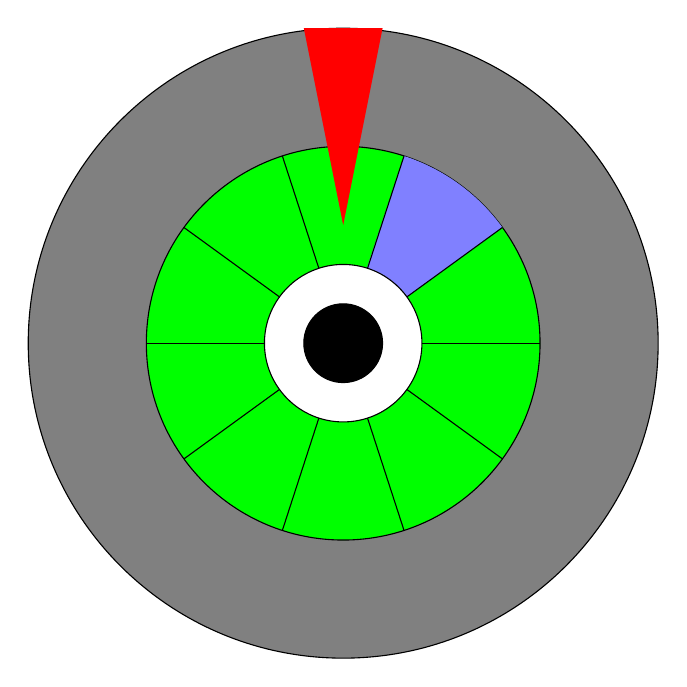
\begin{tikzpicture}
        % Disegna il cerchio esterno
        \fill[gray] (0,0) circle [radius=4];
        \draw (0,0) circle [radius=4];
        
        % Disegna il cerchio intermedio
        \def\radius{2.5}
        \def\n{10}
        \def\angle{360/\n}
        \fill[green] (0,0) circle [radius=\radius];
        \draw (0,0) circle [radius=\radius];

        \foreach \i in {1,...,\n} {
            \ifnum \i=1
                \fill[blue!50] (0.15,0.5) -- (\i*\angle:{0.5}) -- (\i*\angle:{\radius}) arc (\i*\angle:{(\i+1)*\angle}:{\radius}) -- cycle;
            \fi
            \draw (\i*\angle:{0.5}) -- ({\angle * \i}:\radius);
        }

        % Disegna il cerchio interno
        \fill[white] (0,0) circle [radius=1];
        \draw (0,0) circle [radius=1];
        \fill[black] (0,0) circle [radius=0.5];
        \draw (0,0) circle [radius=0.5];     

        % Disegna la testina
        \fill[red] (0,1.5) -- (0.5,4) -- (-0.5,4) -- cycle;
        \end{tikzpicture}
    \end{center}
    \begin{itemize}
        \item \important{Tracce}: superficie in cui l'informazione è memorizzata (colore verde, cerchio intermedio)
        \item \important{Settore}: porzione di traccia (colore blu)
        \item \important{Cilindro}: insieme di tracce allineate verticalmente
        \item \important{Piatto}: colore grigio, cerchio esterno
        \item \important{Asse di rotazione}: asse attorno al quale ruota il piatto in senso orario (colore nero, cerchio interno)
    \end{itemize}
    Un disco è composto da uno o più piatti, per leggere e scrivere utilizza delle testine (una per ogni piatto, nel disegno di colore rosso). Le testine si muovono allo stesso tempo e non sono indipendenti l'una dall'altra.\\
    \remark{Se i dati sono memorizzati su uno stesso cilindro (anche di tracce diverse) possono essere recuperati molto più velocemente che non dati distribuiti su diversi cilindri (il movimento della testina è molto lento).}
    \begin{itemize}
        \item \important{Command Overhead}: tempo impiegato a impartire comandi al drive
        \item \important{Seek Time}: tempo impiegato dal braccio\footnote{Il braccio è quello che tiene tutte le testine allineate} a posizionarsi sulla traccia desiderata
        \item \important{Settle Time}: tempo impiegato per la stabilizzazione del braccio
        \item \important{Rotational Latency}: tempo di attesa dal primo settore da leggere
    \end{itemize}
    \subsection{Tempo di trasferimento}
    Il tempo di trasferimento è il tempo impiegato per trasferire un certo numero di byte e si riferisce alla velocità con cui si trasferiscono byte dai (sui) piatti sulla (dalla) cache del controller. Dipende dalla \important{velocità di trasferimento (o Transfer Rate $Tr$)}.\\
    Un \important{blocco (o pagina)} è una sequenza contigua di settori su una traccia, costituisce l'unità di I/O per il trasferimento dei dati tra il disco e la memoria principale.\\
    Il compito del gestore delle strutture di memorizzazione è quello di ridurre i tempi di latenza.
    \section{Il Database Fisico}
    \important{A livello fisico di un DB consiste in un insieme di file, ognuno dei quali viene visto come una collezione di pagine di dimensione fissa.}
    \begin{center}
        \begin{tabular}{| c | c |}
            \hline
            \textbf{LIVELLO LOGICO} & \textbf{LIVELLO FISICO}\\
            \hline
            Relazione (tabella) & File\\
            \hline
            Tupla & Record\\
            \hline
        \end{tabular}
    \end{center}
    \subsection{File}
    Un file è una sequenza di record, è detto \remark{file con record a lunghezza fissa} se tutti i record hanno la stessa dimensione in byte, altrimenti parliamo di \remark{file con record a lunghezza variabile}.
    \subsection{Record}
    Un record è costituito da un insieme di valori collegati e in generale ogni record include un header che può contenere:
    \begin{itemize}
        \item \important{Identificatore della relazione} cui il record appartiene
        \item \important{Identificatore univoco RID} del record nel DB
        \item \important{Timestamp} che indica quando il record è stato inserito o modificato per l'ultima volta
        \item \important{Lunghezza record}
    \end{itemize}
    \section{Allocazione dei file}
    \subsection{Allocazione contigua}
    \begin{itemize}
        \item I blocchi dei file sono allocati in blocchi di disco contigui quindi non si deve muovere troppo la testina
        \item Rende molto efficiente le letture dell'intero file
        \item Gli aggiornamenti sono costosi (se si ha un file pieno e si vuole aggiungere un record, devo spostare tutti i blocchi in un'altra posizione di lunghezza +1)
    \end{itemize}
    \subsection{Allocazione concatenata}
    \begin{itemize}
        \item Ogni blocco di un file contiene un puntatore al successivo blocco del file
        \item Gli aggiornamenti sono molto efficienti
        \item La lettura dell'intero file è molto lenta
        \item Utilizzo di \important{bucket} non necessariamente contigui ma vicini (possibilmente nello stesso cilindro), per gruppi di record tra loro collegati
    \end{itemize}
    \section{Organizzazione dei record nei file}
    \begin{itemize}
        \item \important{File heap}: i record vengono memorizzati in ordine di inserimento
        \item \important{File ordinato su $X$}: i record vengono memorizzati in ordine rispetto ad un campo $X$
        \item \important{File hash su $X$}: i record vengono memorizzati in ordine parziale rispetto ad un campo $X$ (vengono raggruppati in base al valore di $X$)
    \end{itemize}
    \begin{center}
        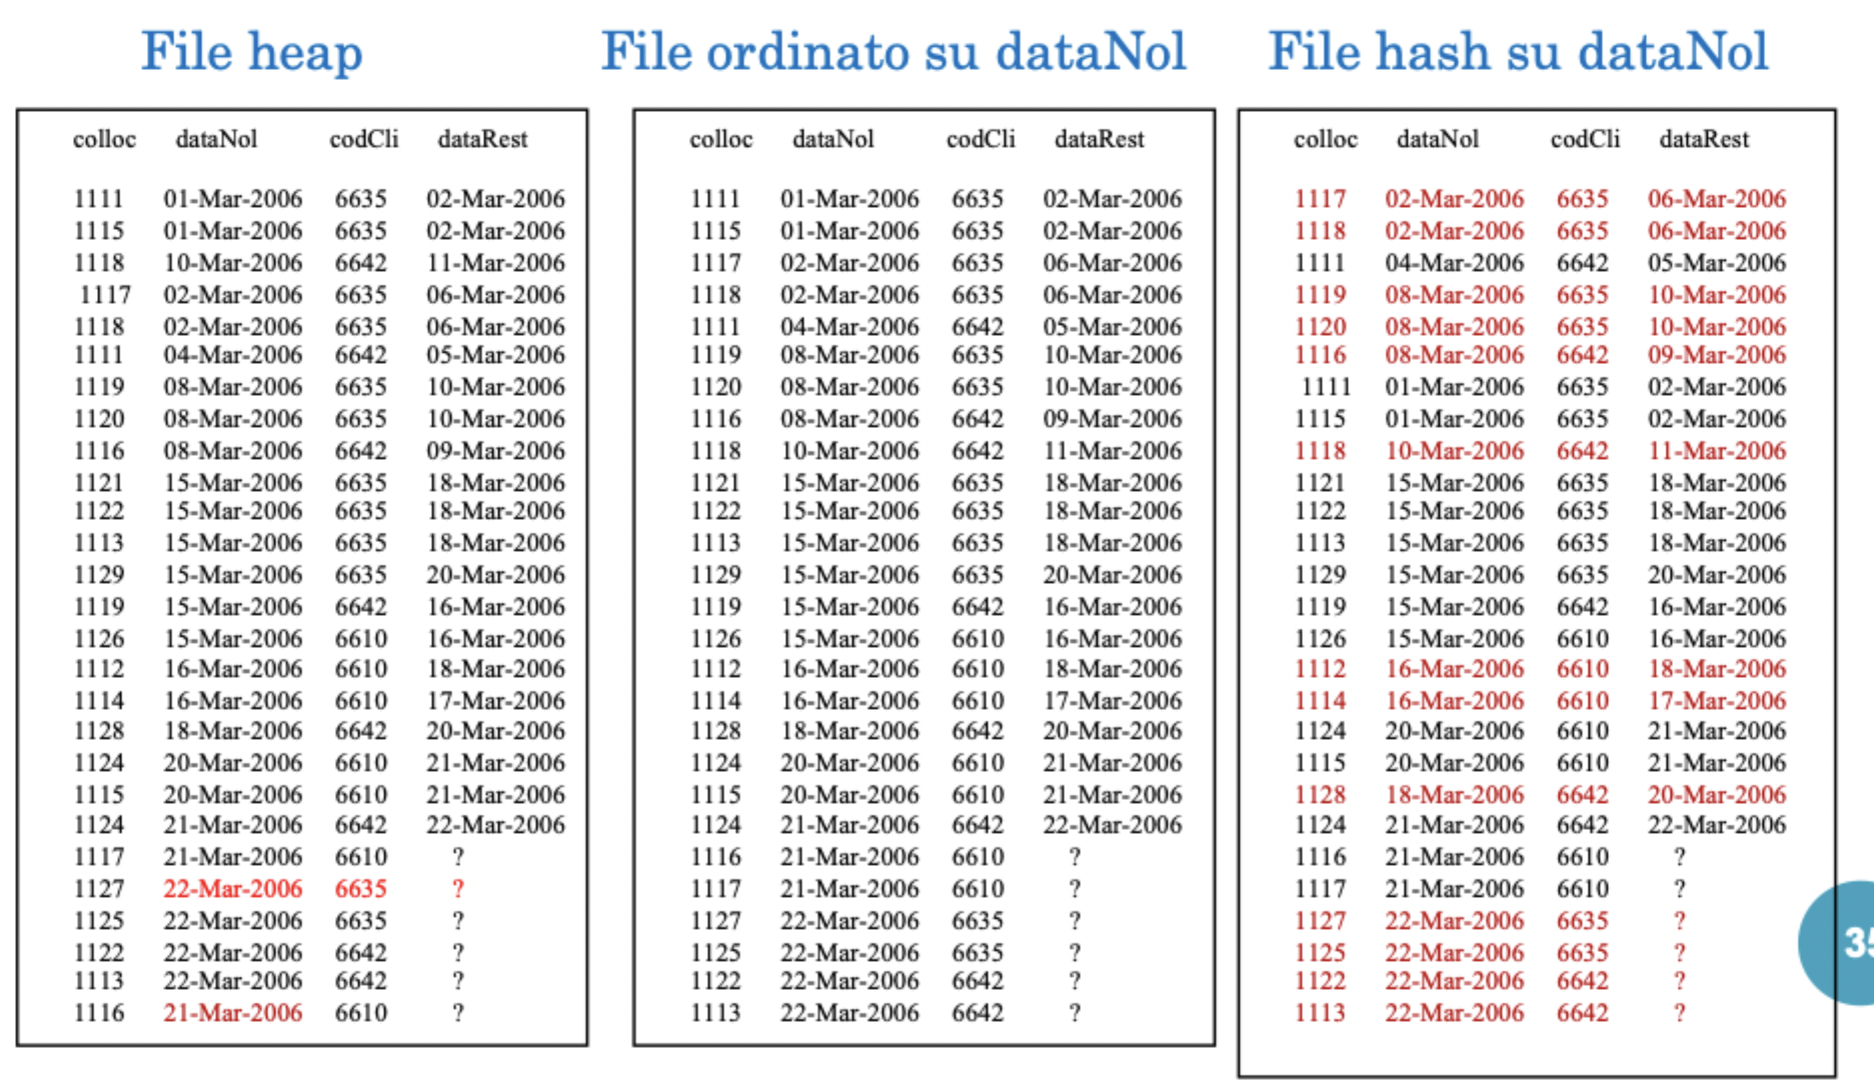
\includegraphics[scale=0.4]{Appunti Latex/Immagini/recordfile.png}
    \end{center}
\end{document}